\documentclass[1p]{elsarticle_modified}
%\bibliographystyle{elsarticle-num}

%\usepackage[colorlinks]{hyperref}
%\usepackage{abbrmath_seonhwa} %\Abb, \Ascr, \Acal ,\Abf, \Afrak
\usepackage{amsfonts}
\usepackage{amssymb}
\usepackage{amsmath}
\usepackage{amsthm}
\usepackage{scalefnt}
\usepackage{amsbsy}
\usepackage{kotex}
\usepackage{caption}
\usepackage{subfig}
\usepackage{color}
\usepackage{graphicx}
\usepackage{xcolor} %% white, black, red, green, blue, cyan, magenta, yellow
\usepackage{float}
\usepackage{setspace}
\usepackage{hyperref}

\usepackage{tikz}
\usetikzlibrary{arrows}

\usepackage{multirow}
\usepackage{array} % fixed length table
\usepackage{hhline}

%%%%%%%%%%%%%%%%%%%%%
\makeatletter
\renewcommand*\env@matrix[1][\arraystretch]{%
	\edef\arraystretch{#1}%
	\hskip -\arraycolsep
	\let\@ifnextchar\new@ifnextchar
	\array{*\c@MaxMatrixCols c}}
\makeatother %https://tex.stackexchange.com/questions/14071/how-can-i-increase-the-line-spacing-in-a-matrix
%%%%%%%%%%%%%%%

\usepackage[normalem]{ulem}

\newcommand{\msout}[1]{\ifmmode\text{\sout{\ensuremath{#1}}}\else\sout{#1}\fi}
%SOURCE: \msout is \stkout macro in https://tex.stackexchange.com/questions/20609/strikeout-in-math-mode

\newcommand{\cancel}[1]{
	\ifmmode
	{\color{red}\msout{#1}}
	\else
	{\color{red}\sout{#1}}
	\fi
}

\newcommand{\add}[1]{
	{\color{blue}\uwave{#1}}
}

\newcommand{\replace}[2]{
	\ifmmode
	{\color{red}\msout{#1}}{\color{blue}\uwave{#2}}
	\else
	{\color{red}\sout{#1}}{\color{blue}\uwave{#2}}
	\fi
}

\newcommand{\Sol}{\mathcal{S}} %segment
\newcommand{\D}{D} %diagram
\newcommand{\A}{\mathcal{A}} %arc


%%%%%%%%%%%%%%%%%%%%%%%%%%%%%5 test

\def\sl{\operatorname{\textup{SL}}(2,\Cbb)}
\def\psl{\operatorname{\textup{PSL}}(2,\Cbb)}
\def\quan{\mkern 1mu \triangleright \mkern 1mu}

\theoremstyle{definition}
\newtheorem{thm}{Theorem}[section]
\newtheorem{prop}[thm]{Proposition}
\newtheorem{lem}[thm]{Lemma}
\newtheorem{ques}[thm]{Question}
\newtheorem{cor}[thm]{Corollary}
\newtheorem{defn}[thm]{Definition}
\newtheorem{exam}[thm]{Example}
\newtheorem{rmk}[thm]{Remark}
\newtheorem{alg}[thm]{Algorithm}

\newcommand{\I}{\sqrt{-1}}
\begin{document}

%\begin{frontmatter}
%
%\title{Boundary parabolic representations of knots up to 8 crossings}
%
%%% Group authors per affiliation:
%\author{Yunhi Cho} 
%\address{Department of Mathematics, University of Seoul, Seoul, Korea}
%\ead{yhcho@uos.ac.kr}
%
%
%\author{Seonhwa Kim} %\fnref{s_kim}}
%\address{Center for Geometry and Physics, Institute for Basic Science, Pohang, 37673, Korea}
%\ead{ryeona17@ibs.re.kr}
%
%\author{Hyuk Kim}
%\address{Department of Mathematical Sciences, Seoul National University, Seoul 08826, Korea}
%\ead{hyukkim@snu.ac.kr}
%
%\author{Seokbeom Yoon}
%\address{Department of Mathematical Sciences, Seoul National University, Seoul, 08826,  Korea}
%\ead{sbyoon15@snu.ac.kr}
%
%\begin{abstract}
%We find all boundary parabolic representation of knots up to 8 crossings.
%
%\end{abstract}
%\begin{keyword}
%    \MSC[2010] 57M25 
%\end{keyword}
%
%\end{frontmatter}

%\linenumbers
%\tableofcontents
%
\newcommand\colored[1]{\textcolor{white}{\rule[-0.35ex]{0.8em}{1.4ex}}\kern-0.8em\color{red} #1}%
%\newcommand\colored[1]{\textcolor{white}{ #1}\kern-2.17ex	\textcolor{white}{ #1}\kern-1.81ex	\textcolor{white}{ #1}\kern-2.15ex\color{red}#1	}

{\Large $\underline{12a_{1271}~(K12a_{1271})}$}

\setlength{\tabcolsep}{10pt}
\renewcommand{\arraystretch}{1.6}
\vspace{1cm}\begin{tabular}{m{100pt}>{\centering\arraybackslash}m{274pt}}
\multirow{5}{120pt}{
	\centering
	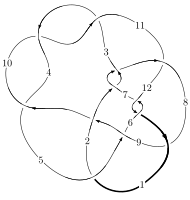
\includegraphics[width=112pt]{../../../GIT/diagram.site/Diagrams/png/2072_12a_1271.png}\\
\ \ \ A knot diagram\footnotemark}&
\allowdisplaybreaks
\textbf{Linearized knot diagam} \\
\cline{2-2}
 &
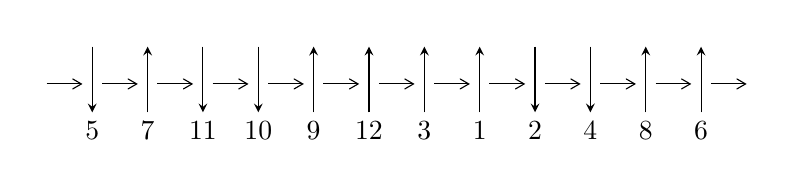
\begin{tikzpicture}[x=20pt, y=17pt]
	% nodes
	\node (C0) at (0, 0) {};
	\node (C1) at (1, 0) {};
	\node (C1U) at (1, +1) {};
	\node (C1D) at (1, -1) {5};

	\node (C2) at (2, 0) {};
	\node (C2U) at (2, +1) {};
	\node (C2D) at (2, -1) {7};

	\node (C3) at (3, 0) {};
	\node (C3U) at (3, +1) {};
	\node (C3D) at (3, -1) {11};

	\node (C4) at (4, 0) {};
	\node (C4U) at (4, +1) {};
	\node (C4D) at (4, -1) {10};

	\node (C5) at (5, 0) {};
	\node (C5U) at (5, +1) {};
	\node (C5D) at (5, -1) {9};

	\node (C6) at (6, 0) {};
	\node (C6U) at (6, +1) {};
	\node (C6D) at (6, -1) {12};

	\node (C7) at (7, 0) {};
	\node (C7U) at (7, +1) {};
	\node (C7D) at (7, -1) {3};

	\node (C8) at (8, 0) {};
	\node (C8U) at (8, +1) {};
	\node (C8D) at (8, -1) {1};

	\node (C9) at (9, 0) {};
	\node (C9U) at (9, +1) {};
	\node (C9D) at (9, -1) {2};

	\node (C10) at (10, 0) {};
	\node (C10U) at (10, +1) {};
	\node (C10D) at (10, -1) {4};

	\node (C11) at (11, 0) {};
	\node (C11U) at (11, +1) {};
	\node (C11D) at (11, -1) {8};

	\node (C12) at (12, 0) {};
	\node (C12U) at (12, +1) {};
	\node (C12D) at (12, -1) {6};
	\node (C13) at (13, 0) {};

	% arrows
	\draw[->,>={angle 60}]
	(C0) edge (C1) (C1) edge (C2) (C2) edge (C3) (C3) edge (C4) (C4) edge (C5) (C5) edge (C6) (C6) edge (C7) (C7) edge (C8) (C8) edge (C9) (C9) edge (C10) (C10) edge (C11) (C11) edge (C12) (C12) edge (C13) ;	\draw[->,>=stealth]
	(C1U) edge (C1D) (C2D) edge (C2U) (C3U) edge (C3D) (C4U) edge (C4D) (C5D) edge (C5U) (C6D) edge (C6U) (C7D) edge (C7U) (C8D) edge (C8U) (C9U) edge (C9D) (C10U) edge (C10D) (C11D) edge (C11U) (C12D) edge (C12U) ;
	\end{tikzpicture} \\
\hhline{~~} \\& 
\textbf{Solving Sequence} \\ \cline{2-2} 
 &
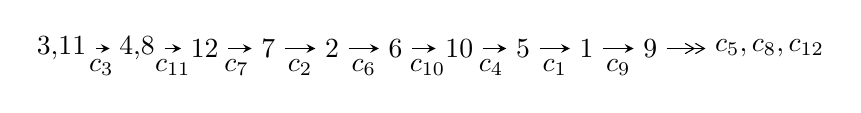
\begin{tikzpicture}[x=23pt, y=7pt]
	% node
	\node (A0) at (-1/8, 0) {3,11};
	\node (A1) at (17/16, 0) {4,8};
	\node (A2) at (17/8, 0) {12};
	\node (A3) at (25/8, 0) {7};
	\node (A4) at (33/8, 0) {2};
	\node (A5) at (41/8, 0) {6};
	\node (A6) at (49/8, 0) {10};
	\node (A7) at (57/8, 0) {5};
	\node (A8) at (65/8, 0) {1};
	\node (A9) at (73/8, 0) {9};
	\node (C1) at (1/2, -1) {$c_{3}$};
	\node (C2) at (13/8, -1) {$c_{11}$};
	\node (C3) at (21/8, -1) {$c_{7}$};
	\node (C4) at (29/8, -1) {$c_{2}$};
	\node (C5) at (37/8, -1) {$c_{6}$};
	\node (C6) at (45/8, -1) {$c_{10}$};
	\node (C7) at (53/8, -1) {$c_{4}$};
	\node (C8) at (61/8, -1) {$c_{1}$};
	\node (C9) at (69/8, -1) {$c_{9}$};
	\node (A10) at (11, 0) {$c_{5},c_{8},c_{12}$};

	% edge
	\draw[->,>=stealth]	
	(A0) edge (A1) (A1) edge (A2) (A2) edge (A3) (A3) edge (A4) (A4) edge (A5) (A5) edge (A6) (A6) edge (A7) (A7) edge (A8) (A8) edge (A9) ;
	\draw[->>,>={angle 60}]	
	(A9) edge (A10);
\end{tikzpicture} \\ 

\end{tabular} \\

\footnotetext{
The image of knot diagram is generated by the software ``\textbf{Draw programme}" developed by Andrew Bartholomew(\url{http://www.layer8.co.uk/maths/draw/index.htm\#Running-draw}), where we modified some parts for our purpose(\url{https://github.com/CATsTAILs/LinksPainter}).
}\phantom \\ \newline 
\centering \textbf{Ideals for irreducible components\footnotemark of $X_{\text{par}}$} 
 
\begin{align*}
I^u_{1}&=\langle 
9.56602\times10^{402} u^{122}+3.14586\times10^{402} u^{121}+\cdots+4.38967\times10^{404} b+9.87332\times10^{404},\\
\phantom{I^u_{1}}&\phantom{= \langle  }4.84508\times10^{405} u^{122}+2.41874\times10^{405} u^{121}+\cdots+1.62418\times10^{406} a-8.32287\times10^{407},\\
\phantom{I^u_{1}}&\phantom{= \langle  }2 u^{123}+u^{122}+\cdots-528 u-37\rangle \\
I^u_{2}&=\langle 
-26117698 u^{27}-222490041 u^{26}+\cdots+494125649 b-12542647,\\
\phantom{I^u_{2}}&\phantom{= \langle  }-124166822468 u^{27}+228098314690 u^{26}+\cdots+64730460019 a-81382930510,\\
\phantom{I^u_{2}}&\phantom{= \langle  }2 u^{28}-3 u^{27}+\cdots-2 u+1\rangle \\
\\
\end{align*}
\raggedright * 2 irreducible components of $\dim_{\mathbb{C}}=0$, with total 151 representations.\\
\footnotetext{All coefficients of polynomials are rational numbers. But the coefficients are sometimes approximated in decimal forms when there is not enough margin.}
\newpage
\renewcommand{\arraystretch}{1}
\centering \section*{I. $I^u_{1}= \langle 9.57\times10^{402} u^{122}+3.15\times10^{402} u^{121}+\cdots+4.39\times10^{404} b+9.87\times10^{404},\;4.85\times10^{405} u^{122}+2.42\times10^{405} u^{121}+\cdots+1.62\times10^{406} a-8.32\times10^{407},\;2 u^{123}+u^{122}+\cdots-528 u-37 \rangle$}
\flushleft \textbf{(i) Arc colorings}\\
\begin{tabular}{m{7pt} m{180pt} m{7pt} m{180pt} }
\flushright $a_{3}=$&$\begin{pmatrix}1\\0\end{pmatrix}$ \\
\flushright $a_{11}=$&$\begin{pmatrix}0\\u\end{pmatrix}$ \\
\flushright $a_{4}=$&$\begin{pmatrix}1\\u^2\end{pmatrix}$ \\
\flushright $a_{8}=$&$\begin{pmatrix}-0.298310 u^{122}-0.148921 u^{121}+\cdots+283.554 u+51.2436\\-0.0217921 u^{122}-0.00716651 u^{121}+\cdots-14.3879 u-2.24922\end{pmatrix}$ \\
\flushright $a_{12}=$&$\begin{pmatrix}0.526224 u^{122}+0.236644 u^{121}+\cdots-452.025 u-77.4936\\0.0515116 u^{122}+0.0404131 u^{121}+\cdots+7.03362 u-0.786561\end{pmatrix}$ \\
\flushright $a_{7}=$&$\begin{pmatrix}-0.276518 u^{122}-0.141755 u^{121}+\cdots+297.942 u+53.4928\\-0.0217921 u^{122}-0.00716651 u^{121}+\cdots-14.3879 u-2.24922\end{pmatrix}$ \\
\flushright $a_{2}=$&$\begin{pmatrix}-0.124303 u^{122}-0.0535248 u^{121}+\cdots+52.5187 u+22.4128\\0.0817857 u^{122}+0.0837779 u^{121}+\cdots-28.5938 u-4.15477\end{pmatrix}$ \\
\flushright $a_{6}=$&$\begin{pmatrix}-0.327328 u^{122}-0.118041 u^{121}+\cdots+326.769 u+48.8014\\-0.0453631 u^{122}-0.00808009 u^{121}+\cdots+38.2331 u+7.37988\end{pmatrix}$ \\
\flushright $a_{10}=$&$\begin{pmatrix}u\\u^3+u\end{pmatrix}$ \\
\flushright $a_{5}=$&$\begin{pmatrix}u^2+1\\u^4+2 u^2\end{pmatrix}$ \\
\flushright $a_{1}=$&$\begin{pmatrix}-0.0591670 u^{122}+0.0181552 u^{121}+\cdots+17.5803 u+17.3490\\0.0804370 u^{122}+0.0582818 u^{121}+\cdots-18.6939 u-3.62441\end{pmatrix}$ \\
\flushright $a_{9}=$&$\begin{pmatrix}0.223915 u^{122}+0.0815103 u^{121}+\cdots-212.003 u-46.3108\\-0.0275443 u^{122}+0.00482334 u^{121}+\cdots+18.8238 u+3.83302\end{pmatrix}$\\&\end{tabular}
\flushleft \textbf{(ii) Obstruction class $= -1$}\\~\\
\flushleft \textbf{(iii) Cusp Shapes $= 0.234910 u^{122}+0.266262 u^{121}+\cdots+98.5953 u+16.9348$}\\~\\
\newpage\renewcommand{\arraystretch}{1}
\flushleft \textbf{(iv) u-Polynomials at the component}\newline \\
\begin{tabular}{m{50pt}|m{274pt}}
Crossings & \hspace{64pt}u-Polynomials at each crossing \\
\hline $$\begin{aligned}c_{1}\end{aligned}$$&$\begin{aligned}
&u^{123}+5 u^{122}+\cdots+10661 u-6658
\end{aligned}$\\
\hline $$\begin{aligned}c_{2},c_{7}\end{aligned}$$&$\begin{aligned}
&u^{123}+3 u^{122}+\cdots+33083 u-2983
\end{aligned}$\\
\hline $$\begin{aligned}c_{3},c_{4},c_{10}\end{aligned}$$&$\begin{aligned}
&2(2 u^{123}+u^{122}+\cdots-528 u-37)
\end{aligned}$\\
\hline $$\begin{aligned}c_{5}\end{aligned}$$&$\begin{aligned}
&2(2 u^{123}-7 u^{122}+\cdots+8241 u-1019)
\end{aligned}$\\
\hline $$\begin{aligned}c_{6},c_{12}\end{aligned}$$&$\begin{aligned}
&2(2 u^{123}+5 u^{122}+\cdots+3232 u-9296)
\end{aligned}$\\
\hline $$\begin{aligned}c_{8}\end{aligned}$$&$\begin{aligned}
&u^{123}+2 u^{122}+\cdots+28 u+1
\end{aligned}$\\
\hline $$\begin{aligned}c_{9}\end{aligned}$$&$\begin{aligned}
&u^{123}-3 u^{122}+\cdots-26333 u+17876
\end{aligned}$\\
\hline $$\begin{aligned}c_{11}\end{aligned}$$&$\begin{aligned}
&u^{123}-3 u^{122}+\cdots-291760059 u+81362762
\end{aligned}$\\
\hline
\end{tabular}\\~\\
\newpage\renewcommand{\arraystretch}{1}
\flushleft \textbf{(v) Riley Polynomials at the component}\newline \\
\begin{tabular}{m{50pt}|m{274pt}}
Crossings & \hspace{64pt}Riley Polynomials at each crossing \\
\hline $$\begin{aligned}c_{1}\end{aligned}$$&$\begin{aligned}
&y^{123}+29 y^{122}+\cdots-1515568995 y-44328964
\end{aligned}$\\
\hline $$\begin{aligned}c_{2},c_{7}\end{aligned}$$&$\begin{aligned}
&y^{123}-77 y^{122}+\cdots-21246601 y-8898289
\end{aligned}$\\
\hline $$\begin{aligned}c_{3},c_{4},c_{10}\end{aligned}$$&$\begin{aligned}
&4(4 y^{123}+535 y^{122}+\cdots+153132 y-1369)
\end{aligned}$\\
\hline $$\begin{aligned}c_{5}\end{aligned}$$&$\begin{aligned}
&4(4 y^{123}+103 y^{122}+\cdots-1.12194\times10^{7} y-1038361)
\end{aligned}$\\
\hline $$\begin{aligned}c_{6},c_{12}\end{aligned}$$&$\begin{aligned}
&4(4 y^{123}+335 y^{122}+\cdots-9.10350\times10^{9} y-8.64156\times10^{7})
\end{aligned}$\\
\hline $$\begin{aligned}c_{8}\end{aligned}$$&$\begin{aligned}
&y^{123}+22 y^{122}+\cdots-540 y-1
\end{aligned}$\\
\hline $$\begin{aligned}c_{9}\end{aligned}$$&$\begin{aligned}
&y^{123}+33 y^{122}+\cdots-10689902655 y-319551376
\end{aligned}$\\
\hline $$\begin{aligned}c_{11}\end{aligned}$$&$\begin{aligned}
&y^{123}-41 y^{122}+\cdots+204460804952227665 y-6619899040268644
\end{aligned}$\\
\hline
\end{tabular}\\~\\
\newpage\flushleft \textbf{(vi) Complex Volumes and Cusp Shapes}
$$\begin{array}{c|c|c}  
\text{Solutions to }I^u_{1}& \I (\text{vol} + \sqrt{-1}CS) & \text{Cusp shape}\\
 \hline 
\begin{aligned}
u &= \phantom{-}0.821306 + 0.575750 I \\
a &= \phantom{-}0.37620 - 1.48100 I \\
b &= \phantom{-}1.177380 - 0.400585 I\end{aligned}
 & \phantom{-}2.48098 - 5.83170 I & \phantom{-0.000000 } 0 \\ \hline\begin{aligned}
u &= \phantom{-}0.821306 - 0.575750 I \\
a &= \phantom{-}0.37620 + 1.48100 I \\
b &= \phantom{-}1.177380 + 0.400585 I\end{aligned}
 & \phantom{-}2.48098 + 5.83170 I & \phantom{-0.000000 } 0 \\ \hline\begin{aligned}
u &= \phantom{-}0.888462 + 0.485693 I \\
a &= -0.484306 + 0.160361 I \\
b &= -1.083620 - 0.079516 I\end{aligned}
 & \phantom{-}2.23175 + 0.42092 I & \phantom{-0.000000 } 0 \\ \hline\begin{aligned}
u &= \phantom{-}0.888462 - 0.485693 I \\
a &= -0.484306 - 0.160361 I \\
b &= -1.083620 + 0.079516 I\end{aligned}
 & \phantom{-}2.23175 - 0.42092 I & \phantom{-0.000000 } 0 \\ \hline\begin{aligned}
u &= -0.065715 + 0.965127 I \\
a &= \phantom{-}0.154437 - 0.645271 I \\
b &= -0.497884 - 0.266752 I\end{aligned}
 & \phantom{-}0.95176 + 1.31743 I & \phantom{-0.000000 } 0 \\ \hline\begin{aligned}
u &= -0.065715 - 0.965127 I \\
a &= \phantom{-}0.154437 + 0.645271 I \\
b &= -0.497884 + 0.266752 I\end{aligned}
 & \phantom{-}0.95176 - 1.31743 I & \phantom{-0.000000 } 0 \\ \hline\begin{aligned}
u &= -0.661126 + 0.696040 I \\
a &= -0.718141 - 0.654042 I \\
b &= -1.071970 + 0.299629 I\end{aligned}
 & -1.04868 - 2.47387 I & \phantom{-0.000000 } 0 \\ \hline\begin{aligned}
u &= -0.661126 - 0.696040 I \\
a &= -0.718141 + 0.654042 I \\
b &= -1.071970 - 0.299629 I\end{aligned}
 & -1.04868 + 2.47387 I & \phantom{-0.000000 } 0 \\ \hline\begin{aligned}
u &= \phantom{-}0.187523 + 0.922512 I \\
a &= \phantom{-}1.071230 - 0.186073 I \\
b &= -0.626268 + 0.492556 I\end{aligned}
 & -2.61548 - 0.66055 I & \phantom{-0.000000 } 0 \\ \hline\begin{aligned}
u &= \phantom{-}0.187523 - 0.922512 I \\
a &= \phantom{-}1.071230 + 0.186073 I \\
b &= -0.626268 - 0.492556 I\end{aligned}
 & -2.61548 + 0.66055 I & \phantom{-0.000000 } 0\\
 \hline 
 \end{array}$$\newpage$$\begin{array}{c|c|c}  
\text{Solutions to }I^u_{1}& \I (\text{vol} + \sqrt{-1}CS) & \text{Cusp shape}\\
 \hline 
\begin{aligned}
u &= \phantom{-}0.483898 + 0.954010 I \\
a &= \phantom{-}0.38199 - 1.61047 I \\
b &= \phantom{-}0.993902 - 0.524937 I\end{aligned}
 & \phantom{-}0.66587 - 1.68115 I & \phantom{-0.000000 } 0 \\ \hline\begin{aligned}
u &= \phantom{-}0.483898 - 0.954010 I \\
a &= \phantom{-}0.38199 + 1.61047 I \\
b &= \phantom{-}0.993902 + 0.524937 I\end{aligned}
 & \phantom{-}0.66587 + 1.68115 I & \phantom{-0.000000 } 0 \\ \hline\begin{aligned}
u &= -0.271344 + 1.055970 I \\
a &= \phantom{-}0.53356 - 1.52032 I \\
b &= \phantom{-}0.752925 - 0.603989 I\end{aligned}
 & -0.08615 - 2.91185 I & \phantom{-0.000000 } 0 \\ \hline\begin{aligned}
u &= -0.271344 - 1.055970 I \\
a &= \phantom{-}0.53356 + 1.52032 I \\
b &= \phantom{-}0.752925 + 0.603989 I\end{aligned}
 & -0.08615 + 2.91185 I & \phantom{-0.000000 } 0 \\ \hline\begin{aligned}
u &= \phantom{-}1.073470 + 0.314108 I \\
a &= \phantom{-}0.816886 + 0.293214 I \\
b &= \phantom{-}1.096480 + 0.357431 I\end{aligned}
 & -1.68259 + 8.21035 I & \phantom{-0.000000 } 0 \\ \hline\begin{aligned}
u &= \phantom{-}1.073470 - 0.314108 I \\
a &= \phantom{-}0.816886 - 0.293214 I \\
b &= \phantom{-}1.096480 - 0.357431 I\end{aligned}
 & -1.68259 - 8.21035 I & \phantom{-0.000000 } 0 \\ \hline\begin{aligned}
u &= \phantom{-}0.824395 + 0.760029 I \\
a &= -0.300542 + 1.344200 I \\
b &= -1.244460 + 0.537834 I\end{aligned}
 & -0.3270 - 14.2808 I & \phantom{-0.000000 } 0 \\ \hline\begin{aligned}
u &= \phantom{-}0.824395 - 0.760029 I \\
a &= -0.300542 - 1.344200 I \\
b &= -1.244460 - 0.537834 I\end{aligned}
 & -0.3270 + 14.2808 I & \phantom{-0.000000 } 0 \\ \hline\begin{aligned}
u &= -0.267435 + 1.099870 I \\
a &= -0.305011 - 0.925898 I \\
b &= -0.876337 - 0.028125 I\end{aligned}
 & \phantom{-}0.956139 + 1.037070 I & \phantom{-0.000000 } 0 \\ \hline\begin{aligned}
u &= -0.267435 - 1.099870 I \\
a &= -0.305011 + 0.925898 I \\
b &= -0.876337 + 0.028125 I\end{aligned}
 & \phantom{-}0.956139 - 1.037070 I & \phantom{-0.000000 } 0\\
 \hline 
 \end{array}$$\newpage$$\begin{array}{c|c|c}  
\text{Solutions to }I^u_{1}& \I (\text{vol} + \sqrt{-1}CS) & \text{Cusp shape}\\
 \hline 
\begin{aligned}
u &= -0.593481 + 0.583322 I \\
a &= -0.191608 + 1.328490 I \\
b &= -0.226497 + 0.989907 I\end{aligned}
 & -3.55874 + 8.80614 I & \phantom{-0.000000 } 0 \\ \hline\begin{aligned}
u &= -0.593481 - 0.583322 I \\
a &= -0.191608 - 1.328490 I \\
b &= -0.226497 - 0.989907 I\end{aligned}
 & -3.55874 - 8.80614 I & \phantom{-0.000000 } 0 \\ \hline\begin{aligned}
u &= -0.474528 + 0.683487 I \\
a &= -0.00586 - 1.45576 I \\
b &= -1.264680 - 0.616575 I\end{aligned}
 & -1.08067 + 5.68283 I & \phantom{-0.000000 } 0 \\ \hline\begin{aligned}
u &= -0.474528 - 0.683487 I \\
a &= -0.00586 + 1.45576 I \\
b &= -1.264680 + 0.616575 I\end{aligned}
 & -1.08067 - 5.68283 I & \phantom{-0.000000 } 0 \\ \hline\begin{aligned}
u &= -0.670345 + 0.454387 I \\
a &= \phantom{-}0.75109 + 1.35319 I \\
b &= \phantom{-}1.237040 + 0.531743 I\end{aligned}
 & -1.67033 + 7.04459 I & \phantom{-0.000000 } 0 \\ \hline\begin{aligned}
u &= -0.670345 - 0.454387 I \\
a &= \phantom{-}0.75109 - 1.35319 I \\
b &= \phantom{-}1.237040 - 0.531743 I\end{aligned}
 & -1.67033 - 7.04459 I & \phantom{-0.000000 } 0 \\ \hline\begin{aligned}
u &= -0.889063 + 0.824559 I \\
a &= \phantom{-}0.339799 + 0.832689 I \\
b &= \phantom{-}1.198440 + 0.293277 I\end{aligned}
 & \phantom{-}4.42995 + 7.73324 I & \phantom{-0.000000 } 0 \\ \hline\begin{aligned}
u &= -0.889063 - 0.824559 I \\
a &= \phantom{-}0.339799 - 0.832689 I \\
b &= \phantom{-}1.198440 - 0.293277 I\end{aligned}
 & \phantom{-}4.42995 - 7.73324 I & \phantom{-0.000000 } 0 \\ \hline\begin{aligned}
u &= \phantom{-}0.762334 + 0.145940 I \\
a &= -1.76251 - 0.77310 I \\
b &= -0.959387 - 0.322392 I\end{aligned}
 & -1.82052 - 2.70790 I & \phantom{-0.000000 } 0 \\ \hline\begin{aligned}
u &= \phantom{-}0.762334 - 0.145940 I \\
a &= -1.76251 + 0.77310 I \\
b &= -0.959387 + 0.322392 I\end{aligned}
 & -1.82052 + 2.70790 I & \phantom{-0.000000 } 0\\
 \hline 
 \end{array}$$\newpage$$\begin{array}{c|c|c}  
\text{Solutions to }I^u_{1}& \I (\text{vol} + \sqrt{-1}CS) & \text{Cusp shape}\\
 \hline 
\begin{aligned}
u &= \phantom{-}0.771558\phantom{ +0.000000I} \\
a &= -1.05154\phantom{ +0.000000I} \\
b &= -1.28315\phantom{ +0.000000I}\end{aligned}
 & \phantom{-}2.74555\phantom{ +0.000000I} & \phantom{-0.000000 } 0 \\ \hline\begin{aligned}
u &= \phantom{-}0.343892 + 0.684932 I \\
a &= -0.133429 - 0.606375 I \\
b &= -0.996989 - 0.434157 I\end{aligned}
 & \phantom{-}2.03687 + 1.43581 I & \phantom{-0.000000 } 0 \\ \hline\begin{aligned}
u &= \phantom{-}0.343892 - 0.684932 I \\
a &= -0.133429 + 0.606375 I \\
b &= -0.996989 + 0.434157 I\end{aligned}
 & \phantom{-}2.03687 - 1.43581 I & \phantom{-0.000000 } 0 \\ \hline\begin{aligned}
u &= -0.613227 + 0.433414 I \\
a &= -1.28627 + 1.14789 I \\
b &= \phantom{-}0.312298 + 0.492561 I\end{aligned}
 & -4.04362 - 4.68912 I & \phantom{-0.000000 } 0 \\ \hline\begin{aligned}
u &= -0.613227 - 0.433414 I \\
a &= -1.28627 - 1.14789 I \\
b &= \phantom{-}0.312298 - 0.492561 I\end{aligned}
 & -4.04362 + 4.68912 I & \phantom{-0.000000 } 0 \\ \hline\begin{aligned}
u &= -0.566231 + 0.467381 I \\
a &= \phantom{-}0.429439 - 1.303690 I \\
b &= \phantom{-}0.070394 - 0.640386 I\end{aligned}
 & -0.74627 + 1.87969 I & \phantom{-0.000000 } 0 \\ \hline\begin{aligned}
u &= -0.566231 - 0.467381 I \\
a &= \phantom{-}0.429439 + 1.303690 I \\
b &= \phantom{-}0.070394 + 0.640386 I\end{aligned}
 & -0.74627 - 1.87969 I & \phantom{-0.000000 } 0 \\ \hline\begin{aligned}
u &= \phantom{-}0.373666 + 0.569590 I \\
a &= \phantom{-}0.675317 - 0.628063 I \\
b &= -0.151756 - 0.121172 I\end{aligned}
 & \phantom{-}1.19060 + 0.97150 I & \phantom{-0.000000 } 0 \\ \hline\begin{aligned}
u &= \phantom{-}0.373666 - 0.569590 I \\
a &= \phantom{-}0.675317 + 0.628063 I \\
b &= -0.151756 + 0.121172 I\end{aligned}
 & \phantom{-}1.19060 - 0.97150 I & \phantom{-0.000000 } 0 \\ \hline\begin{aligned}
u &= \phantom{-}0.508121 + 0.438554 I \\
a &= -0.549978 + 1.064350 I \\
b &= -0.075671 + 0.706568 I\end{aligned}
 & \phantom{-}0.64905 - 4.26495 I & \phantom{-0.000000 -}0. + 7.73497 I\\
 \hline 
 \end{array}$$\newpage$$\begin{array}{c|c|c}  
\text{Solutions to }I^u_{1}& \I (\text{vol} + \sqrt{-1}CS) & \text{Cusp shape}\\
 \hline 
\begin{aligned}
u &= \phantom{-}0.508121 - 0.438554 I \\
a &= -0.549978 - 1.064350 I \\
b &= -0.075671 - 0.706568 I\end{aligned}
 & \phantom{-}0.64905 + 4.26495 I & \phantom{-0.000000 } 0. - 7.73497 I \\ \hline\begin{aligned}
u &= \phantom{-}0.234565 + 1.308270 I \\
a &= \phantom{-}1.021150 - 0.224599 I \\
b &= \phantom{-}0.910078 + 0.078208 I\end{aligned}
 & \phantom{-}2.65265 - 6.28084 I & \phantom{-0.000000 } 0 \\ \hline\begin{aligned}
u &= \phantom{-}0.234565 - 1.308270 I \\
a &= \phantom{-}1.021150 + 0.224599 I \\
b &= \phantom{-}0.910078 - 0.078208 I\end{aligned}
 & \phantom{-}2.65265 + 6.28084 I & \phantom{-0.000000 } 0 \\ \hline\begin{aligned}
u &= \phantom{-}0.399348 + 0.538165 I \\
a &= -0.757600 - 1.096510 I \\
b &= \phantom{-}1.108070 - 0.326234 I\end{aligned}
 & \phantom{-}1.73412 - 4.24811 I & \phantom{-0.000000 -}0. + 6.74904 I \\ \hline\begin{aligned}
u &= \phantom{-}0.399348 - 0.538165 I \\
a &= -0.757600 + 1.096510 I \\
b &= \phantom{-}1.108070 + 0.326234 I\end{aligned}
 & \phantom{-}1.73412 + 4.24811 I & \phantom{-0.000000 } 0. - 6.74904 I \\ \hline\begin{aligned}
u &= \phantom{-}0.022247 + 0.645132 I \\
a &= \phantom{-}0.243797 + 0.889141 I \\
b &= \phantom{-}1.355980 + 0.006009 I\end{aligned}
 & \phantom{-}2.52785 - 5.12439 I & \phantom{-}7.37684 + 6.09074 I \\ \hline\begin{aligned}
u &= \phantom{-}0.022247 - 0.645132 I \\
a &= \phantom{-}0.243797 - 0.889141 I \\
b &= \phantom{-}1.355980 - 0.006009 I\end{aligned}
 & \phantom{-}2.52785 + 5.12439 I & \phantom{-}7.37684 - 6.09074 I \\ \hline\begin{aligned}
u &= \phantom{-}0.300977 + 0.554618 I \\
a &= \phantom{-}0.24267 - 2.19815 I \\
b &= \phantom{-}1.170580 - 0.089071 I\end{aligned}
 & \phantom{-}4.86680 - 1.87555 I & \phantom{-}12.89229 + 3.77881 I \\ \hline\begin{aligned}
u &= \phantom{-}0.300977 - 0.554618 I \\
a &= \phantom{-}0.24267 + 2.19815 I \\
b &= \phantom{-}1.170580 + 0.089071 I\end{aligned}
 & \phantom{-}4.86680 + 1.87555 I & \phantom{-}12.89229 - 3.77881 I \\ \hline\begin{aligned}
u &= -0.233026 + 1.373320 I \\
a &= -0.478285 - 0.027672 I \\
b &= -0.076126 + 0.216418 I\end{aligned}
 & \phantom{-}4.01446 + 4.15866 I & \phantom{-0.000000 } 0\\
 \hline 
 \end{array}$$\newpage$$\begin{array}{c|c|c}  
\text{Solutions to }I^u_{1}& \I (\text{vol} + \sqrt{-1}CS) & \text{Cusp shape}\\
 \hline 
\begin{aligned}
u &= -0.233026 - 1.373320 I \\
a &= -0.478285 + 0.027672 I \\
b &= -0.076126 - 0.216418 I\end{aligned}
 & \phantom{-}4.01446 - 4.15866 I & \phantom{-0.000000 } 0 \\ \hline\begin{aligned}
u &= -0.566398 + 0.215733 I \\
a &= \phantom{-}0.641030 - 0.721225 I \\
b &= \phantom{-}0.122104 - 0.449288 I\end{aligned}
 & -0.99237 + 1.19266 I & -2.78479 - 1.90364 I \\ \hline\begin{aligned}
u &= -0.566398 - 0.215733 I \\
a &= \phantom{-}0.641030 + 0.721225 I \\
b &= \phantom{-}0.122104 + 0.449288 I\end{aligned}
 & -0.99237 - 1.19266 I & -2.78479 + 1.90364 I \\ \hline\begin{aligned}
u &= -0.587969 + 0.117877 I \\
a &= \phantom{-}1.66498 + 0.00661 I \\
b &= \phantom{-}0.949537 - 0.431732 I\end{aligned}
 & -2.67680 - 2.15681 I & -2.19591 + 3.12767 I \\ \hline\begin{aligned}
u &= -0.587969 - 0.117877 I \\
a &= \phantom{-}1.66498 - 0.00661 I \\
b &= \phantom{-}0.949537 + 0.431732 I\end{aligned}
 & -2.67680 + 2.15681 I & -2.19591 - 3.12767 I \\ \hline\begin{aligned}
u &= -0.09306 + 1.41750 I \\
a &= \phantom{-}1.202790 - 0.574115 I \\
b &= -1.026960 + 0.044437 I\end{aligned}
 & \phantom{-}1.54486 - 1.39803 I & \phantom{-0.000000 } 0 \\ \hline\begin{aligned}
u &= -0.09306 - 1.41750 I \\
a &= \phantom{-}1.202790 + 0.574115 I \\
b &= -1.026960 - 0.044437 I\end{aligned}
 & \phantom{-}1.54486 + 1.39803 I & \phantom{-0.000000 } 0 \\ \hline\begin{aligned}
u &= -0.06443 + 1.43813 I \\
a &= -0.277602 - 1.195840 I \\
b &= -0.807021 - 0.789461 I\end{aligned}
 & \phantom{-}1.81995 + 2.92375 I & \phantom{-0.000000 } 0 \\ \hline\begin{aligned}
u &= -0.06443 - 1.43813 I \\
a &= -0.277602 + 1.195840 I \\
b &= -0.807021 + 0.789461 I\end{aligned}
 & \phantom{-}1.81995 - 2.92375 I & \phantom{-0.000000 } 0 \\ \hline\begin{aligned}
u &= \phantom{-}0.168847 + 0.525271 I \\
a &= -1.38296 - 0.41894 I \\
b &= \phantom{-}0.477482 - 0.817206 I\end{aligned}
 & -3.94878 - 2.48873 I & -2.37089 + 7.95153 I\\
 \hline 
 \end{array}$$\newpage$$\begin{array}{c|c|c}  
\text{Solutions to }I^u_{1}& \I (\text{vol} + \sqrt{-1}CS) & \text{Cusp shape}\\
 \hline 
\begin{aligned}
u &= \phantom{-}0.168847 - 0.525271 I \\
a &= -1.38296 + 0.41894 I \\
b &= \phantom{-}0.477482 + 0.817206 I\end{aligned}
 & -3.94878 + 2.48873 I & -2.37089 - 7.95153 I \\ \hline\begin{aligned}
u &= \phantom{-}0.05698 + 1.46259 I \\
a &= -0.108076 - 0.667046 I \\
b &= -0.35426 - 1.46772 I\end{aligned}
 & \phantom{-}0.89120 - 2.50465 I & \phantom{-0.000000 } 0 \\ \hline\begin{aligned}
u &= \phantom{-}0.05698 - 1.46259 I \\
a &= -0.108076 + 0.667046 I \\
b &= -0.35426 + 1.46772 I\end{aligned}
 & \phantom{-}0.89120 + 2.50465 I & \phantom{-0.000000 } 0 \\ \hline\begin{aligned}
u &= -0.09232 + 1.48608 I \\
a &= -1.95091 - 0.06714 I \\
b &= \phantom{-}1.027050 + 0.044735 I\end{aligned}
 & \phantom{-}3.02811 + 6.76823 I & \phantom{-0.000000 } 0 \\ \hline\begin{aligned}
u &= -0.09232 - 1.48608 I \\
a &= -1.95091 + 0.06714 I \\
b &= \phantom{-}1.027050 - 0.044735 I\end{aligned}
 & \phantom{-}3.02811 - 6.76823 I & \phantom{-0.000000 } 0 \\ \hline\begin{aligned}
u &= \phantom{-}0.17406 + 1.47983 I \\
a &= -0.448160 - 0.740634 I \\
b &= \phantom{-}1.51152 - 0.26912 I\end{aligned}
 & \phantom{-}8.14515 - 3.17570 I & \phantom{-0.000000 } 0 \\ \hline\begin{aligned}
u &= \phantom{-}0.17406 - 1.47983 I \\
a &= -0.448160 + 0.740634 I \\
b &= \phantom{-}1.51152 + 0.26912 I\end{aligned}
 & \phantom{-}8.14515 + 3.17570 I & \phantom{-0.000000 } 0 \\ \hline\begin{aligned}
u &= -0.19565 + 1.51130 I \\
a &= \phantom{-}0.402349 - 1.020670 I \\
b &= -1.45443 - 0.68152 I\end{aligned}
 & \phantom{-}4.78994 + 10.10650 I & \phantom{-0.000000 } 0 \\ \hline\begin{aligned}
u &= -0.19565 - 1.51130 I \\
a &= \phantom{-}0.402349 + 1.020670 I \\
b &= -1.45443 + 0.68152 I\end{aligned}
 & \phantom{-}4.78994 - 10.10650 I & \phantom{-0.000000 } 0 \\ \hline\begin{aligned}
u &= -0.08241 + 1.52199 I \\
a &= -0.80125 + 1.27457 I \\
b &= \phantom{-}1.37281 + 0.47552 I\end{aligned}
 & \phantom{-}8.14920 + 7.12933 I & \phantom{-0.000000 } 0\\
 \hline 
 \end{array}$$\newpage$$\begin{array}{c|c|c}  
\text{Solutions to }I^u_{1}& \I (\text{vol} + \sqrt{-1}CS) & \text{Cusp shape}\\
 \hline 
\begin{aligned}
u &= -0.08241 - 1.52199 I \\
a &= -0.80125 - 1.27457 I \\
b &= \phantom{-}1.37281 - 0.47552 I\end{aligned}
 & \phantom{-}8.14920 - 7.12933 I & \phantom{-0.000000 } 0 \\ \hline\begin{aligned}
u &= -0.17770 + 1.51407 I \\
a &= -0.320304 + 0.682712 I \\
b &= -0.060148 + 0.961871 I\end{aligned}
 & \phantom{-}5.79302 + 4.58086 I & \phantom{-0.000000 } 0 \\ \hline\begin{aligned}
u &= -0.17770 - 1.51407 I \\
a &= -0.320304 - 0.682712 I \\
b &= -0.060148 - 0.961871 I\end{aligned}
 & \phantom{-}5.79302 - 4.58086 I & \phantom{-0.000000 } 0 \\ \hline\begin{aligned}
u &= \phantom{-}0.03560 + 1.52587 I \\
a &= \phantom{-}0.152006 + 0.493142 I \\
b &= \phantom{-}0.20270 + 1.59077 I\end{aligned}
 & \phantom{-}2.01880 - 0.12358 I & \phantom{-0.000000 } 0 \\ \hline\begin{aligned}
u &= \phantom{-}0.03560 - 1.52587 I \\
a &= \phantom{-}0.152006 - 0.493142 I \\
b &= \phantom{-}0.20270 - 1.59077 I\end{aligned}
 & \phantom{-}2.01880 + 0.12358 I & \phantom{-0.000000 } 0 \\ \hline\begin{aligned}
u &= \phantom{-}0.14189 + 1.52038 I \\
a &= -0.016213 - 0.755114 I \\
b &= \phantom{-}0.232193 - 1.171810 I\end{aligned}
 & \phantom{-}7.20225 - 6.53938 I & \phantom{-0.000000 } 0 \\ \hline\begin{aligned}
u &= \phantom{-}0.14189 - 1.52038 I \\
a &= -0.016213 + 0.755114 I \\
b &= \phantom{-}0.232193 + 1.171810 I\end{aligned}
 & \phantom{-}7.20225 + 6.53938 I & \phantom{-0.000000 } 0 \\ \hline\begin{aligned}
u &= \phantom{-}0.02531 + 1.52740 I \\
a &= -0.316151 - 0.836586 I \\
b &= \phantom{-}1.47650 - 0.67300 I\end{aligned}
 & \phantom{-}10.97280 - 0.40185 I & \phantom{-0.000000 } 0 \\ \hline\begin{aligned}
u &= \phantom{-}0.02531 - 1.52740 I \\
a &= -0.316151 + 0.836586 I \\
b &= \phantom{-}1.47650 + 0.67300 I\end{aligned}
 & \phantom{-}10.97280 + 0.40185 I & \phantom{-0.000000 } 0 \\ \hline\begin{aligned}
u &= -0.221269 + 0.402394 I \\
a &= \phantom{-}0.54033 - 3.57089 I \\
b &= -1.298420 - 0.315444 I\end{aligned}
 & \phantom{-}1.56498 + 5.97171 I & \phantom{-}11.86443 - 6.77214 I\\
 \hline 
 \end{array}$$\newpage$$\begin{array}{c|c|c}  
\text{Solutions to }I^u_{1}& \I (\text{vol} + \sqrt{-1}CS) & \text{Cusp shape}\\
 \hline 
\begin{aligned}
u &= -0.221269 - 0.402394 I \\
a &= \phantom{-}0.54033 + 3.57089 I \\
b &= -1.298420 + 0.315444 I\end{aligned}
 & \phantom{-}1.56498 - 5.97171 I & \phantom{-}11.86443 + 6.77214 I \\ \hline\begin{aligned}
u &= \phantom{-}0.11128 + 1.53725 I \\
a &= -0.097438 + 0.746880 I \\
b &= -0.014743 + 0.796330 I\end{aligned}
 & \phantom{-}8.12667 - 0.76838 I & \phantom{-0.000000 } 0 \\ \hline\begin{aligned}
u &= \phantom{-}0.11128 - 1.53725 I \\
a &= -0.097438 - 0.746880 I \\
b &= -0.014743 - 0.796330 I\end{aligned}
 & \phantom{-}8.12667 + 0.76838 I & \phantom{-0.000000 } 0 \\ \hline\begin{aligned}
u &= -0.05951 + 1.55007 I \\
a &= \phantom{-}0.504350 + 0.433865 I \\
b &= -0.266714 + 0.792997 I\end{aligned}
 & \phantom{-}3.26304 - 2.31319 I & \phantom{-0.000000 } 0 \\ \hline\begin{aligned}
u &= -0.05951 - 1.55007 I \\
a &= \phantom{-}0.504350 - 0.433865 I \\
b &= -0.266714 - 0.792997 I\end{aligned}
 & \phantom{-}3.26304 + 2.31319 I & \phantom{-0.000000 } 0 \\ \hline\begin{aligned}
u &= \phantom{-}0.238605 + 0.370889 I \\
a &= -0.712947 - 1.130240 I \\
b &= -0.227745 - 1.243130 I\end{aligned}
 & -4.49862 + 0.65916 I & -3.09576 + 6.41157 I \\ \hline\begin{aligned}
u &= \phantom{-}0.238605 - 0.370889 I \\
a &= -0.712947 + 1.130240 I \\
b &= -0.227745 + 1.243130 I\end{aligned}
 & -4.49862 - 0.65916 I & -3.09576 - 6.41157 I \\ \hline\begin{aligned}
u &= \phantom{-}0.08576 + 1.55702 I \\
a &= \phantom{-}0.523575 + 1.103580 I \\
b &= -1.275700 + 0.344537 I\end{aligned}
 & \phantom{-}12.03740 - 3.28062 I & \phantom{-0.000000 } 0 \\ \hline\begin{aligned}
u &= \phantom{-}0.08576 - 1.55702 I \\
a &= \phantom{-}0.523575 - 1.103580 I \\
b &= -1.275700 - 0.344537 I\end{aligned}
 & \phantom{-}12.03740 + 3.28062 I & \phantom{-0.000000 } 0 \\ \hline\begin{aligned}
u &= \phantom{-}0.156686 + 0.411401 I \\
a &= -0.90478 + 2.30137 I \\
b &= -1.279530 + 0.343200 I\end{aligned}
 & \phantom{-}4.30555 + 0.12568 I & \phantom{-}11.56781 - 3.17091 I\\
 \hline 
 \end{array}$$\newpage$$\begin{array}{c|c|c}  
\text{Solutions to }I^u_{1}& \I (\text{vol} + \sqrt{-1}CS) & \text{Cusp shape}\\
 \hline 
\begin{aligned}
u &= \phantom{-}0.156686 - 0.411401 I \\
a &= -0.90478 - 2.30137 I \\
b &= -1.279530 - 0.343200 I\end{aligned}
 & \phantom{-}4.30555 - 0.12568 I & \phantom{-}11.56781 + 3.17091 I \\ \hline\begin{aligned}
u &= \phantom{-}0.02703 + 1.56361 I \\
a &= \phantom{-}0.482876 - 0.394798 I \\
b &= -1.57890 - 0.26314 I\end{aligned}
 & \phantom{-}10.00810 - 5.45882 I & \phantom{-0.000000 } 0 \\ \hline\begin{aligned}
u &= \phantom{-}0.02703 - 1.56361 I \\
a &= \phantom{-}0.482876 + 0.394798 I \\
b &= -1.57890 + 0.26314 I\end{aligned}
 & \phantom{-}10.00810 + 5.45882 I & \phantom{-0.000000 } 0 \\ \hline\begin{aligned}
u &= -0.18290 + 1.55908 I \\
a &= \phantom{-}0.241042 - 0.677384 I \\
b &= \phantom{-}0.163547 - 1.308400 I\end{aligned}
 & \phantom{-}3.58353 + 11.64840 I & \phantom{-0.000000 } 0 \\ \hline\begin{aligned}
u &= -0.18290 - 1.55908 I \\
a &= \phantom{-}0.241042 + 0.677384 I \\
b &= \phantom{-}0.163547 + 1.308400 I\end{aligned}
 & \phantom{-}3.58353 - 11.64840 I & \phantom{-0.000000 } 0 \\ \hline\begin{aligned}
u &= \phantom{-}0.11834 + 1.57169 I \\
a &= \phantom{-}0.775920 + 0.486481 I \\
b &= -1.43829 + 0.30576 I\end{aligned}
 & \phantom{-}8.97050 - 6.12397 I & \phantom{-0.000000 } 0 \\ \hline\begin{aligned}
u &= \phantom{-}0.11834 - 1.57169 I \\
a &= \phantom{-}0.775920 - 0.486481 I \\
b &= -1.43829 - 0.30576 I\end{aligned}
 & \phantom{-}8.97050 + 6.12397 I & \phantom{-0.000000 } 0 \\ \hline\begin{aligned}
u &= \phantom{-}0.01624 + 1.59222 I \\
a &= -0.383853 + 0.507771 I \\
b &= \phantom{-}1.35022 + 0.48512 I\end{aligned}
 & \phantom{-}10.03810 + 0.59329 I & \phantom{-0.000000 } 0 \\ \hline\begin{aligned}
u &= \phantom{-}0.01624 - 1.59222 I \\
a &= -0.383853 - 0.507771 I \\
b &= \phantom{-}1.35022 - 0.48512 I\end{aligned}
 & \phantom{-}10.03810 - 0.59329 I & \phantom{-0.000000 } 0 \\ \hline\begin{aligned}
u &= -0.13667 + 1.59487 I \\
a &= -0.595570 + 0.848522 I \\
b &= \phantom{-}1.51331 + 0.66571 I\end{aligned}
 & \phantom{-}6.62792 + 7.94764 I & \phantom{-0.000000 } 0\\
 \hline 
 \end{array}$$\newpage$$\begin{array}{c|c|c}  
\text{Solutions to }I^u_{1}& \I (\text{vol} + \sqrt{-1}CS) & \text{Cusp shape}\\
 \hline 
\begin{aligned}
u &= -0.13667 - 1.59487 I \\
a &= -0.595570 - 0.848522 I \\
b &= \phantom{-}1.51331 - 0.66571 I\end{aligned}
 & \phantom{-}6.62792 - 7.94764 I & \phantom{-0.000000 } 0 \\ \hline\begin{aligned}
u &= \phantom{-}0.28986 + 1.57463 I \\
a &= \phantom{-}0.436738 + 1.283910 I \\
b &= -1.292140 + 0.537051 I\end{aligned}
 & \phantom{-}9.53392 - 9.97126 I & \phantom{-0.000000 } 0 \\ \hline\begin{aligned}
u &= \phantom{-}0.28986 - 1.57463 I \\
a &= \phantom{-}0.436738 - 1.283910 I \\
b &= -1.292140 - 0.537051 I\end{aligned}
 & \phantom{-}9.53392 + 9.97126 I & \phantom{-0.000000 } 0 \\ \hline\begin{aligned}
u &= -0.332578 + 0.210309 I \\
a &= \phantom{-}3.99857 - 3.82161 I \\
b &= -0.740612 - 0.225976 I\end{aligned}
 & -2.84248 + 5.34682 I & \phantom{-}3.0402 - 14.1291 I \\ \hline\begin{aligned}
u &= -0.332578 - 0.210309 I \\
a &= \phantom{-}3.99857 + 3.82161 I \\
b &= -0.740612 + 0.225976 I\end{aligned}
 & -2.84248 - 5.34682 I & \phantom{-}3.0402 + 14.1291 I \\ \hline\begin{aligned}
u &= \phantom{-}0.319557 + 0.205174 I \\
a &= -0.17587 + 2.00836 I \\
b &= \phantom{-}0.339040 + 1.087230 I\end{aligned}
 & -4.73999 - 1.38888 I & -8.18552 + 9.20306 I \\ \hline\begin{aligned}
u &= \phantom{-}0.319557 - 0.205174 I \\
a &= -0.17587 - 2.00836 I \\
b &= \phantom{-}0.339040 - 1.087230 I\end{aligned}
 & -4.73999 + 1.38888 I & -8.18552 - 9.20306 I \\ \hline\begin{aligned}
u &= -0.11614 + 1.63623 I \\
a &= -0.395934 + 0.811509 I \\
b &= \phantom{-}1.029910 + 0.053937 I\end{aligned}
 & \phantom{-}7.22204 + 0.26579 I & \phantom{-0.000000 } 0 \\ \hline\begin{aligned}
u &= -0.11614 - 1.63623 I \\
a &= -0.395934 - 0.811509 I \\
b &= \phantom{-}1.029910 - 0.053937 I\end{aligned}
 & \phantom{-}7.22204 - 0.26579 I & \phantom{-0.000000 } 0 \\ \hline\begin{aligned}
u &= \phantom{-}0.05770 + 1.64687 I \\
a &= \phantom{-}0.142205 + 0.940817 I \\
b &= -1.112710 + 0.827183 I\end{aligned}
 & \phantom{-}9.79001 - 3.28548 I & \phantom{-0.000000 } 0\\
 \hline 
 \end{array}$$\newpage$$\begin{array}{c|c|c}  
\text{Solutions to }I^u_{1}& \I (\text{vol} + \sqrt{-1}CS) & \text{Cusp shape}\\
 \hline 
\begin{aligned}
u &= \phantom{-}0.05770 - 1.64687 I \\
a &= \phantom{-}0.142205 - 0.940817 I \\
b &= -1.112710 - 0.827183 I\end{aligned}
 & \phantom{-}9.79001 + 3.28548 I & \phantom{-0.000000 } 0 \\ \hline\begin{aligned}
u &= \phantom{-}0.33263 + 1.61856 I \\
a &= -0.267522 - 0.549377 I \\
b &= \phantom{-}1.357130 - 0.112709 I\end{aligned}
 & \phantom{-}9.09350 - 4.31625 I & \phantom{-0.000000 } 0 \\ \hline\begin{aligned}
u &= \phantom{-}0.33263 - 1.61856 I \\
a &= -0.267522 + 0.549377 I \\
b &= \phantom{-}1.357130 + 0.112709 I\end{aligned}
 & \phantom{-}9.09350 + 4.31625 I & \phantom{-0.000000 } 0 \\ \hline\begin{aligned}
u &= \phantom{-}0.27065 + 1.63011 I \\
a &= -0.424432 - 1.115910 I \\
b &= \phantom{-}1.39250 - 0.63595 I\end{aligned}
 & \phantom{-}7.5621 - 18.4218 I & \phantom{-0.000000 } 0 \\ \hline\begin{aligned}
u &= \phantom{-}0.27065 - 1.63011 I \\
a &= -0.424432 + 1.115910 I \\
b &= \phantom{-}1.39250 + 0.63595 I\end{aligned}
 & \phantom{-}7.5621 + 18.4218 I & \phantom{-0.000000 } 0 \\ \hline\begin{aligned}
u &= -0.27178 + 1.64321 I \\
a &= \phantom{-}0.334443 - 0.876866 I \\
b &= -1.42910 - 0.44346 I\end{aligned}
 & \phantom{-}12.5393 + 12.0640 I & \phantom{-0.000000 } 0 \\ \hline\begin{aligned}
u &= -0.27178 - 1.64321 I \\
a &= \phantom{-}0.334443 + 0.876866 I \\
b &= -1.42910 + 0.44346 I\end{aligned}
 & \phantom{-}12.5393 - 12.0640 I & \phantom{-0.000000 } 0 \\ \hline\begin{aligned}
u &= -0.27220 + 1.68723 I \\
a &= -0.307776 + 0.853779 I \\
b &= \phantom{-}1.272740 + 0.391980 I\end{aligned}
 & \phantom{-}12.12140 + 5.05912 I & \phantom{-0.000000 } 0 \\ \hline\begin{aligned}
u &= -0.27220 - 1.68723 I \\
a &= -0.307776 - 0.853779 I \\
b &= \phantom{-}1.272740 - 0.391980 I\end{aligned}
 & \phantom{-}12.12140 - 5.05912 I & \phantom{-0.000000 } 0 \\ \hline\begin{aligned}
u &= -0.1150270 + 0.0115063 I \\
a &= \phantom{-}7.93172 + 7.13213 I \\
b &= \phantom{-}0.798573 - 0.513973 I\end{aligned}
 & -3.22439 - 2.14554 I & -4.98018 + 3.72211 I\\
 \hline 
 \end{array}$$\newpage$$\begin{array}{c|c|c}  
\text{Solutions to }I^u_{1}& \I (\text{vol} + \sqrt{-1}CS) & \text{Cusp shape}\\
 \hline 
\begin{aligned}
u &= -0.1150270 - 0.0115063 I \\
a &= \phantom{-}7.93172 - 7.13213 I \\
b &= \phantom{-}0.798573 + 0.513973 I\end{aligned}
 & -3.22439 + 2.14554 I & -4.98018 - 3.72211 I \\ \hline\begin{aligned}
u &= -1.61350 + 1.21787 I \\
a &= -0.111943 - 0.304491 I \\
b &= -1.021780 - 0.049257 I\end{aligned}
 & \phantom{-}3.15370 - 0.16077 I & \phantom{-0.000000 } 0 \\ \hline\begin{aligned}
u &= -1.61350 - 1.21787 I \\
a &= -0.111943 + 0.304491 I \\
b &= -1.021780 + 0.049257 I\end{aligned}
 & \phantom{-}3.15370 + 0.16077 I & \phantom{-0.000000 } 0\\
 \hline 
 \end{array}$$\newpage\newpage\renewcommand{\arraystretch}{1}
\centering \section*{II. $I^u_{2}= \langle -2.61\times10^{7} u^{27}-2.22\times10^{8} u^{26}+\cdots+4.94\times10^{8} b-1.25\times10^{7},\;-1.24\times10^{11} u^{27}+2.28\times10^{11} u^{26}+\cdots+6.47\times10^{10} a-8.14\times10^{10},\;2 u^{28}-3 u^{27}+\cdots-2 u+1 \rangle$}
\flushleft \textbf{(i) Arc colorings}\\
\begin{tabular}{m{7pt} m{180pt} m{7pt} m{180pt} }
\flushright $a_{3}=$&$\begin{pmatrix}1\\0\end{pmatrix}$ \\
\flushright $a_{11}=$&$\begin{pmatrix}0\\u\end{pmatrix}$ \\
\flushright $a_{4}=$&$\begin{pmatrix}1\\u^2\end{pmatrix}$ \\
\flushright $a_{8}=$&$\begin{pmatrix}1.91821 u^{27}-3.52382 u^{26}+\cdots+4.63300 u+1.25726\\0.0528564 u^{27}+0.450270 u^{26}+\cdots+4.66394 u+0.0253835\end{pmatrix}$ \\
\flushright $a_{12}=$&$\begin{pmatrix}0.0263085 u^{27}-0.711609 u^{26}+\cdots+3.99013 u-3.32024\\-0.253249 u^{27}+0.321752 u^{26}+\cdots-0.453641 u-0.176542\end{pmatrix}$ \\
\flushright $a_{7}=$&$\begin{pmatrix}1.86536 u^{27}-3.97409 u^{26}+\cdots-0.0309420 u+1.23188\\0.0528564 u^{27}+0.450270 u^{26}+\cdots+4.66394 u+0.0253835\end{pmatrix}$ \\
\flushright $a_{2}=$&$\begin{pmatrix}0.204718 u^{27}-0.577219 u^{26}+\cdots+8.42236 u+0.546407\\0.148365 u^{27}-0.205654 u^{26}+\cdots+1.64754 u-1.35313\end{pmatrix}$ \\
\flushright $a_{6}=$&$\begin{pmatrix}-1.15147 u^{27}+3.49656 u^{26}+\cdots-7.12765 u+1.76057\\-0.621442 u^{27}+2.21400 u^{26}+\cdots+1.10324 u+0.528788\end{pmatrix}$ \\
\flushright $a_{10}=$&$\begin{pmatrix}u\\u^3+u\end{pmatrix}$ \\
\flushright $a_{5}=$&$\begin{pmatrix}u^2+1\\u^4+2 u^2\end{pmatrix}$ \\
\flushright $a_{1}=$&$\begin{pmatrix}-0.0325227 u^{27}-0.311472 u^{26}+\cdots+10.5638 u-0.866160\\0.414757 u^{27}-0.204393 u^{26}+\cdots+1.53617 u-1.16284\end{pmatrix}$ \\
\flushright $a_{9}=$&$\begin{pmatrix}1.04252 u^{27}-2.42103 u^{26}+\cdots+2.58820 u-2.44844\\-0.309396 u^{27}+0.991119 u^{26}+\cdots-4.52599 u+1.31563\end{pmatrix}$\\&\end{tabular}
\flushleft \textbf{(ii) Obstruction class $= 1$}\\~\\
\flushleft \textbf{(iii) Cusp Shapes $= \frac{180472544174}{64730460019} u^{27}-\frac{129321336473}{64730460019} u^{26}+\cdots+\frac{1092503506402}{64730460019} u+\frac{291508413369}{64730460019}$}\\~\\
\newpage\renewcommand{\arraystretch}{1}
\flushleft \textbf{(iv) u-Polynomials at the component}\newline \\
\begin{tabular}{m{50pt}|m{274pt}}
Crossings & \hspace{64pt}u-Polynomials at each crossing \\
\hline $$\begin{aligned}c_{1}\end{aligned}$$&$\begin{aligned}
&u^{28}+2 u^{27}+\cdots+7 u+2
\end{aligned}$\\
\hline $$\begin{aligned}c_{2}\end{aligned}$$&$\begin{aligned}
&u^{28}-2 u^{27}+\cdots- u+1
\end{aligned}$\\
\hline $$\begin{aligned}c_{3},c_{4}\end{aligned}$$&$\begin{aligned}
&2(2 u^{28}-3 u^{27}+\cdots-2 u+1)
\end{aligned}$\\
\hline $$\begin{aligned}c_{5}\end{aligned}$$&$\begin{aligned}
&2(2 u^{28}-7 u^{27}+\cdots-5 u+1)
\end{aligned}$\\
\hline $$\begin{aligned}c_{6}\end{aligned}$$&$\begin{aligned}
&2(2 u^{28}-3 u^{27}+\cdots+16 u+4)
\end{aligned}$\\
\hline $$\begin{aligned}c_{7}\end{aligned}$$&$\begin{aligned}
&u^{28}+2 u^{27}+\cdots+u+1
\end{aligned}$\\
\hline $$\begin{aligned}c_{8}\end{aligned}$$&$\begin{aligned}
&u^{28}- u^{27}+\cdots+2 u+1
\end{aligned}$\\
\hline $$\begin{aligned}c_{9}\end{aligned}$$&$\begin{aligned}
&u^{28}+9 u^{26}+\cdots-35 u+4
\end{aligned}$\\
\hline $$\begin{aligned}c_{10}\end{aligned}$$&$\begin{aligned}
&2(2 u^{28}+3 u^{27}+\cdots+2 u+1)
\end{aligned}$\\
\hline $$\begin{aligned}c_{11}\end{aligned}$$&$\begin{aligned}
&u^{28}+2 u^{26}+\cdots-61 u+14
\end{aligned}$\\
\hline $$\begin{aligned}c_{12}\end{aligned}$$&$\begin{aligned}
&2(2 u^{28}+3 u^{27}+\cdots-16 u+4)
\end{aligned}$\\
\hline
\end{tabular}\\~\\
\newpage\renewcommand{\arraystretch}{1}
\flushleft \textbf{(v) Riley Polynomials at the component}\newline \\
\begin{tabular}{m{50pt}|m{274pt}}
Crossings & \hspace{64pt}Riley Polynomials at each crossing \\
\hline $$\begin{aligned}c_{1}\end{aligned}$$&$\begin{aligned}
&y^{28}+2 y^{27}+\cdots+19 y+4
\end{aligned}$\\
\hline $$\begin{aligned}c_{2},c_{7}\end{aligned}$$&$\begin{aligned}
&y^{28}-12 y^{27}+\cdots-19 y+1
\end{aligned}$\\
\hline $$\begin{aligned}c_{3},c_{4},c_{10}\end{aligned}$$&$\begin{aligned}
&4(4 y^{28}+123 y^{27}+\cdots+32 y+1)
\end{aligned}$\\
\hline $$\begin{aligned}c_{5}\end{aligned}$$&$\begin{aligned}
&4(4 y^{28}+27 y^{27}+\cdots+9 y+1)
\end{aligned}$\\
\hline $$\begin{aligned}c_{6},c_{12}\end{aligned}$$&$\begin{aligned}
&4(4 y^{28}+83 y^{27}+\cdots+96 y+16)
\end{aligned}$\\
\hline $$\begin{aligned}c_{8}\end{aligned}$$&$\begin{aligned}
&y^{28}+23 y^{27}+\cdots-12 y+1
\end{aligned}$\\
\hline $$\begin{aligned}c_{9}\end{aligned}$$&$\begin{aligned}
&y^{28}+18 y^{27}+\cdots-785 y+16
\end{aligned}$\\
\hline $$\begin{aligned}c_{11}\end{aligned}$$&$\begin{aligned}
&y^{28}+4 y^{27}+\cdots+647 y+196
\end{aligned}$\\
\hline
\end{tabular}\\~\\
\newpage\flushleft \textbf{(vi) Complex Volumes and Cusp Shapes}
$$\begin{array}{c|c|c}  
\text{Solutions to }I^u_{2}& \I (\text{vol} + \sqrt{-1}CS) & \text{Cusp shape}\\
 \hline 
\begin{aligned}
u &= -0.008025 + 1.095820 I \\
a &= \phantom{-}0.64035 + 1.63660 I \\
b &= \phantom{-}0.812859 + 0.564856 I\end{aligned}
 & -0.98996 + 2.29936 I & -1.47584 - 2.11904 I \\ \hline\begin{aligned}
u &= -0.008025 - 1.095820 I \\
a &= \phantom{-}0.64035 - 1.63660 I \\
b &= \phantom{-}0.812859 - 0.564856 I\end{aligned}
 & -0.98996 - 2.29936 I & -1.47584 + 2.11904 I \\ \hline\begin{aligned}
u &= \phantom{-}1.171530 + 0.135101 I \\
a &= -0.661586 + 0.104382 I \\
b &= -1.130320 + 0.029289 I\end{aligned}
 & \phantom{-}3.04675 + 0.00214 I & \phantom{-}16.8127 + 1.5074 I \\ \hline\begin{aligned}
u &= \phantom{-}1.171530 - 0.135101 I \\
a &= -0.661586 - 0.104382 I \\
b &= -1.130320 - 0.029289 I\end{aligned}
 & \phantom{-}3.04675 - 0.00214 I & \phantom{-}16.8127 - 1.5074 I \\ \hline\begin{aligned}
u &= -0.307913 + 0.753218 I \\
a &= \phantom{-}0.285067 + 0.817010 I \\
b &= -0.888623 + 0.368385 I\end{aligned}
 & \phantom{-}2.17371 - 2.01469 I & \phantom{-}9.57123 + 7.54695 I \\ \hline\begin{aligned}
u &= -0.307913 - 0.753218 I \\
a &= \phantom{-}0.285067 - 0.817010 I \\
b &= -0.888623 - 0.368385 I\end{aligned}
 & \phantom{-}2.17371 + 2.01469 I & \phantom{-}9.57123 - 7.54695 I \\ \hline\begin{aligned}
u &= -0.132754 + 0.736721 I \\
a &= \phantom{-}0.790140 - 1.075570 I \\
b &= -0.873273 + 0.438007 I\end{aligned}
 & -2.29537 - 1.87184 I & \phantom{-}2.98347 + 3.16131 I \\ \hline\begin{aligned}
u &= -0.132754 - 0.736721 I \\
a &= \phantom{-}0.790140 + 1.075570 I \\
b &= -0.873273 - 0.438007 I\end{aligned}
 & -2.29537 + 1.87184 I & \phantom{-}2.98347 - 3.16131 I \\ \hline\begin{aligned}
u &= \phantom{-}0.003285 + 1.273060 I \\
a &= \phantom{-}0.539557 + 0.331923 I \\
b &= -0.055302 + 0.758594 I\end{aligned}
 & -0.87252 + 1.15187 I & -1.27136 - 1.43599 I \\ \hline\begin{aligned}
u &= \phantom{-}0.003285 - 1.273060 I \\
a &= \phantom{-}0.539557 - 0.331923 I \\
b &= -0.055302 - 0.758594 I\end{aligned}
 & -0.87252 - 1.15187 I & -1.27136 + 1.43599 I\\
 \hline 
 \end{array}$$\newpage$$\begin{array}{c|c|c}  
\text{Solutions to }I^u_{2}& \I (\text{vol} + \sqrt{-1}CS) & \text{Cusp shape}\\
 \hline 
\begin{aligned}
u &= -0.215698 + 1.297370 I \\
a &= \phantom{-}0.388654 - 0.001676 I \\
b &= \phantom{-}0.606066 + 0.226952 I\end{aligned}
 & \phantom{-}4.47887 + 4.56895 I & \phantom{-}10.77443 - 6.54974 I \\ \hline\begin{aligned}
u &= -0.215698 - 1.297370 I \\
a &= \phantom{-}0.388654 + 0.001676 I \\
b &= \phantom{-}0.606066 - 0.226952 I\end{aligned}
 & \phantom{-}4.47887 - 4.56895 I & \phantom{-}10.77443 + 6.54974 I \\ \hline\begin{aligned}
u &= \phantom{-}0.137397 + 1.370990 I \\
a &= -1.59911 + 0.16102 I \\
b &= -0.440357 + 0.139322 I\end{aligned}
 & \phantom{-}1.45021 - 6.68619 I & -0.19760 + 6.34878 I \\ \hline\begin{aligned}
u &= \phantom{-}0.137397 - 1.370990 I \\
a &= -1.59911 - 0.16102 I \\
b &= -0.440357 - 0.139322 I\end{aligned}
 & \phantom{-}1.45021 + 6.68619 I & -0.19760 - 6.34878 I \\ \hline\begin{aligned}
u &= -0.488137 + 0.345385 I \\
a &= \phantom{-}0.38002 + 2.26602 I \\
b &= \phantom{-}1.283430 + 0.347849 I\end{aligned}
 & \phantom{-}0.83358 + 6.07227 I & \phantom{-}0.02294 - 8.71575 I \\ \hline\begin{aligned}
u &= -0.488137 - 0.345385 I \\
a &= \phantom{-}0.38002 - 2.26602 I \\
b &= \phantom{-}1.283430 - 0.347849 I\end{aligned}
 & \phantom{-}0.83358 - 6.07227 I & \phantom{-}0.02294 + 8.71575 I \\ \hline\begin{aligned}
u &= -0.00156 + 1.51798 I \\
a &= -0.214119 - 0.525739 I \\
b &= -0.06460 - 1.49850 I\end{aligned}
 & \phantom{-}1.98118 - 1.14085 I & \phantom{-}1.67149 + 4.55352 I \\ \hline\begin{aligned}
u &= -0.00156 - 1.51798 I \\
a &= -0.214119 + 0.525739 I \\
b &= -0.06460 + 1.49850 I\end{aligned}
 & \phantom{-}1.98118 + 1.14085 I & \phantom{-}1.67149 - 4.55352 I \\ \hline\begin{aligned}
u &= -0.13204 + 1.55089 I \\
a &= \phantom{-}0.784150 - 0.957831 I \\
b &= -1.49170 - 0.50620 I\end{aligned}
 & \phantom{-}7.46841 + 8.20050 I & \phantom{-}7.14741 - 8.88305 I \\ \hline\begin{aligned}
u &= -0.13204 - 1.55089 I \\
a &= \phantom{-}0.784150 + 0.957831 I \\
b &= -1.49170 + 0.50620 I\end{aligned}
 & \phantom{-}7.46841 - 8.20050 I & \phantom{-}7.14741 + 8.88305 I\\
 \hline 
 \end{array}$$\newpage$$\begin{array}{c|c|c}  
\text{Solutions to }I^u_{2}& \I (\text{vol} + \sqrt{-1}CS) & \text{Cusp shape}\\
 \hline 
\begin{aligned}
u &= \phantom{-}0.409316 + 0.122472 I \\
a &= -0.44720 - 4.23815 I \\
b &= \phantom{-}0.599807 + 0.096913 I\end{aligned}
 & -2.88784 + 4.85383 I & \phantom{-}2.58432 + 0.86409 I \\ \hline\begin{aligned}
u &= \phantom{-}0.409316 - 0.122472 I \\
a &= -0.44720 + 4.23815 I \\
b &= \phantom{-}0.599807 - 0.096913 I\end{aligned}
 & -2.88784 - 4.85383 I & \phantom{-}2.58432 - 0.86409 I \\ \hline\begin{aligned}
u &= \phantom{-}0.23735 + 1.56199 I \\
a &= -0.426922 - 0.578032 I \\
b &= \phantom{-}1.41544 - 0.16291 I\end{aligned}
 & \phantom{-}8.54980 - 4.07721 I & \phantom{-}2.00000 + 3.73465 I \\ \hline\begin{aligned}
u &= \phantom{-}0.23735 - 1.56199 I \\
a &= -0.426922 + 0.578032 I \\
b &= \phantom{-}1.41544 + 0.16291 I\end{aligned}
 & \phantom{-}8.54980 + 4.07721 I & \phantom{-}2.00000 - 3.73465 I \\ \hline\begin{aligned}
u &= \phantom{-}0.07930 + 1.59683 I \\
a &= -0.273069 - 0.923398 I \\
b &= \phantom{-}1.171420 - 0.582185 I\end{aligned}
 & \phantom{-}10.95870 - 2.55041 I & \phantom{-}9.71429 + 0. I\phantom{ +0.000000I} \\ \hline\begin{aligned}
u &= \phantom{-}0.07930 - 1.59683 I \\
a &= -0.273069 + 0.923398 I \\
b &= \phantom{-}1.171420 + 0.582185 I\end{aligned}
 & \phantom{-}10.95870 + 2.55041 I & \phantom{-}9.71429 + 0. I\phantom{ +0.000000I} \\ \hline\begin{aligned}
u &= -0.002061 + 0.255353 I \\
a &= \phantom{-}1.81406 + 0.98908 I \\
b &= \phantom{-}0.055155 + 1.174080 I\end{aligned}
 & -4.28671 - 1.15758 I & \phantom{-}5.54668 + 4.43189 I \\ \hline\begin{aligned}
u &= -0.002061 - 0.255353 I \\
a &= \phantom{-}1.81406 - 0.98908 I \\
b &= \phantom{-}0.055155 - 1.174080 I\end{aligned}
 & -4.28671 + 1.15758 I & \phantom{-}5.54668 - 4.43189 I\\
 \hline 
 \end{array}$$\newpage
\newpage\renewcommand{\arraystretch}{1}
\centering \section*{ III. u-Polynomials}
\begin{tabular}{m{50pt}|m{274pt}}
Crossings & \hspace{64pt}u-Polynomials at each crossing \\
\hline $$\begin{aligned}c_{1}\end{aligned}$$&$\begin{aligned}
&(u^{28}+2 u^{27}+\cdots+7 u+2)(u^{123}+5 u^{122}+\cdots+10661 u-6658)
\end{aligned}$\\
\hline $$\begin{aligned}c_{2}\end{aligned}$$&$\begin{aligned}
&(u^{28}-2 u^{27}+\cdots- u+1)(u^{123}+3 u^{122}+\cdots+33083 u-2983)
\end{aligned}$\\
\hline $$\begin{aligned}c_{3},c_{4}\end{aligned}$$&$\begin{aligned}
&4(2 u^{28}-3 u^{27}+\cdots-2 u+1)(2 u^{123}+u^{122}+\cdots-528 u-37)
\end{aligned}$\\
\hline $$\begin{aligned}c_{5}\end{aligned}$$&$\begin{aligned}
&4(2 u^{28}-7 u^{27}+\cdots-5 u+1)(2 u^{123}-7 u^{122}+\cdots+8241 u-1019)
\end{aligned}$\\
\hline $$\begin{aligned}c_{6}\end{aligned}$$&$\begin{aligned}
&4(2 u^{28}-3 u^{27}+\cdots+16 u+4)(2 u^{123}+5 u^{122}+\cdots+3232 u-9296)
\end{aligned}$\\
\hline $$\begin{aligned}c_{7}\end{aligned}$$&$\begin{aligned}
&(u^{28}+2 u^{27}+\cdots+u+1)(u^{123}+3 u^{122}+\cdots+33083 u-2983)
\end{aligned}$\\
\hline $$\begin{aligned}c_{8}\end{aligned}$$&$\begin{aligned}
&(u^{28}- u^{27}+\cdots+2 u+1)(u^{123}+2 u^{122}+\cdots+28 u+1)
\end{aligned}$\\
\hline $$\begin{aligned}c_{9}\end{aligned}$$&$\begin{aligned}
&(u^{28}+9 u^{26}+\cdots-35 u+4)(u^{123}-3 u^{122}+\cdots-26333 u+17876)
\end{aligned}$\\
\hline $$\begin{aligned}c_{10}\end{aligned}$$&$\begin{aligned}
&4(2 u^{28}+3 u^{27}+\cdots+2 u+1)(2 u^{123}+u^{122}+\cdots-528 u-37)
\end{aligned}$\\
\hline $$\begin{aligned}c_{11}\end{aligned}$$&$\begin{aligned}
&(u^{28}+2 u^{26}+\cdots-61 u+14)\\
&\cdot(u^{123}-3 u^{122}+\cdots-291760059 u+81362762)
\end{aligned}$\\
\hline $$\begin{aligned}c_{12}\end{aligned}$$&$\begin{aligned}
&4(2 u^{28}+3 u^{27}+\cdots-16 u+4)(2 u^{123}+5 u^{122}+\cdots+3232 u-9296)
\end{aligned}$\\
\hline
\end{tabular}\newpage\renewcommand{\arraystretch}{1}
\centering \section*{ IV. Riley Polynomials}
\begin{tabular}{m{50pt}|m{274pt}}
Crossings & \hspace{64pt}Riley Polynomials at each crossing \\
\hline $$\begin{aligned}c_{1}\end{aligned}$$&$\begin{aligned}
&(y^{28}+2 y^{27}+\cdots+19 y+4)\\
&\cdot(y^{123}+29 y^{122}+\cdots-1515568995 y-44328964)
\end{aligned}$\\
\hline $$\begin{aligned}c_{2},c_{7}\end{aligned}$$&$\begin{aligned}
&(y^{28}-12 y^{27}+\cdots-19 y+1)\\
&\cdot(y^{123}-77 y^{122}+\cdots-21246601 y-8898289)
\end{aligned}$\\
\hline $$\begin{aligned}c_{3},c_{4},c_{10}\end{aligned}$$&$\begin{aligned}
&16(4 y^{28}+123 y^{27}+\cdots+32 y+1)\\
&\cdot(4 y^{123}+535 y^{122}+\cdots+153132 y-1369)
\end{aligned}$\\
\hline $$\begin{aligned}c_{5}\end{aligned}$$&$\begin{aligned}
&16(4 y^{28}+27 y^{27}+\cdots+9 y+1)\\
&\cdot(4 y^{123}+103 y^{122}+\cdots-11219421 y-1038361)
\end{aligned}$\\
\hline $$\begin{aligned}c_{6},c_{12}\end{aligned}$$&$\begin{aligned}
&16(4 y^{28}+83 y^{27}+\cdots+96 y+16)\\
&\cdot(4 y^{123}+335 y^{122}+\cdots-9103501312 y-86415616)
\end{aligned}$\\
\hline $$\begin{aligned}c_{8}\end{aligned}$$&$\begin{aligned}
&(y^{28}+23 y^{27}+\cdots-12 y+1)(y^{123}+22 y^{122}+\cdots-540 y-1)
\end{aligned}$\\
\hline $$\begin{aligned}c_{9}\end{aligned}$$&$\begin{aligned}
&(y^{28}+18 y^{27}+\cdots-785 y+16)\\
&\cdot(y^{123}+33 y^{122}+\cdots-10689902655 y-319551376)
\end{aligned}$\\
\hline $$\begin{aligned}c_{11}\end{aligned}$$&$\begin{aligned}
&(y^{28}+4 y^{27}+\cdots+647 y+196)\\
&\cdot(y^{123}-41 y^{122}+\cdots+204460804952227665 y-6619899040268644)
\end{aligned}$\\
\hline
\end{tabular}
\vskip 2pc
\end{document}